% !TEX root = ../my-thesis.tex
%
\chapter{Empirical Analysis and Evaluation}
\label{sec:evaluation}
After devising the approach for optimizer ensembles and implementing it as a reference implementation, it is essential to evaluate and assess this approach.
This assessment is the goal of this chapter and the final step of this thesis.\newline
The evaluated reference implementation is nicknamed \textit{frankensteins-automl}, because this AutoML approach is metaphorically stitched together from different optimizers like Frankenstein's Monster.
It will henceforth be referenced by this name while describing the experiment setup as well as listing and evaluating the experiment results.

To have a clear guided structure for this assessment of frankensteins-automl, it is based on the research questions presented in section~\ref{sec:intro:goal}, which are elucidated here in more detail at first.
This more detailed elucidation of the research questions has a focus on which data is required to answer the corresponding question.\newline
Afterwards, this chapter explains a series of Empirical evaluations in the form of experiments to gather this required data.
Therefore, the setup and configuration of the experiments are given as part of these explanations.\newline
Subsequently, the outcomes of the experiments are presented and analyzed to deduce the answers to the research questions from them.

\section{Research Questions in Detail}
The first research question is about the feasibility of the approach, i.e. is it a viable idea to optimize an AutoML problem solution with an optimizer ensemble.
This will be answered in two steps.\newline
At first, are the solution scores of this approach similar to or better than the scores of other state-of-the-art approaches for several different datasets?
If they are not similar/better at all or not similar/better for a high number of datasets, frankensteins-automl is not a competitor to the state-of-the-art approaches.
In this case, there would be no motivation to use this approach instead of other approaches, until this approach is further enhanced and the scores have improved.\newline
Second, if there is an improvement in some scores, which of the two components of the approach, the MCTS model selection or the warmstarted optimizer ensemble model configuration, had which influence on the resulting scores.
To assess these influences, three versions of frankensteins-automl are evaluated, where two of them have slight modifications:
\begin{enumerate}
    \item To evaluate the influence of a Model Selection via an MCTS, this modified version does not utilize an optimizer ensemble.
    Every optimizer node represents the same optimizer, which is a wamrstarted SMAC for this evaluation.
    In the remaining chapter it will be referenced as \textit{frankenstein-mcts.}
    \item To evaluate the influence of the ensembled optimizers, this modified version does not utilize an UCT based node selection.
    The node selection on each level down the paths to the different optimizer nodes, is random for each search iteration.
    Therefore, it is basically a repeated random search.
    Hence, it will be named \textit{frankenstein-rs}.
    \item The original and unmodified \textit{frankensteins-automl} as described in the two previous chapters with an MCTS and optimizer ensembles with all five optimization algorithms.
\end{enumerate}
By comparing the scores of the three variants for different datasets and different timeouts, data about the scores with and without one component can be gathered, which can be used to analyze the influence of the component.

As the second research question, the focus lies on the utilization of the different optimizers.
During each run of frankensteins-automl it is counted how many times each optimizer was selected by the MCTS and therewith an optimization run with this optimizer started.
Since the MCTS tries to find the best suited optimizer and to exploit it, this selection frequency could be an indicator of the suitability of this optimizer to the input dataset.\newline
The frequencies are aggregated together with the properties of the AutoML input dataset.
Thus, it is possible to check if one or more optimizers were preferably selected in general for all settings, i.e. for all datasets, or just in an AutoML problem setting with a certain input dataset that has certain properties.
Alternatively, there could be no significant difference and each optimizer is selected comparably often across all observed AutoML settings, or one or more optimizer are used primarily unrelated to the dataset.

\section{Experiment Setup}
\label{sec:evaluation:setup}
To answer the first step of the first research question, frankensteins-automl is benchmarked against different other competitor state-of-the-art approaches.
The selection of these approaches is made to represent the different established optimization strategies in the current state-of-the-art.\newline
\textit{ML-Plan} is selected for optimization via searching, \textit{TPOT} as an approach with a genetic algorithm, \textit{auto-sklearn} for Bayesian optimization, and finally \textit{Mosaic} as a related work approach that utilizes more than one optimization method via an optimization space transformation.\newline
Since ML-Plan is the only approach out of this selection, which is not implemented in Python but in Java, it can not be integrated seamlessly in the same experimental setup as the remaining ones.
The experimental results for ML-Plan were kindly provided by the original authors of the approach~\textcite{Mohr-ML-Plan}.
All other approaches will be evaluated in a unified Python experiment environment that is explained in more detail in Appendix~\ref{sec:appendix:singularity}.

The experimental setup has a certain set of constraints and rules, which are enforced equally for all approaches to achieve a fair and meaningful comparison
They are summarized in the following:
\begin{enumerate}
    \item Each AutoML experiment setting (i.e. a combination of dataset + timeout + approach) will be conducted with 30 different random seeds to achieve a better statistical robustness against outliers in the evaluation scores.
    \item The different approaches have 60 Gb RAM and 16 CPU cores, Intel Xeon E5-2670 with 2.6 Ghz, as a hardware limitation.
    \item A pipeline candidate evaluation during the AutoML process, i.e. constructing, training and testing a candidate, must not take longer than five minutes and will be terminated otherwise.
    \item All AutoML approaches will utilize the model selection and configuration space from auto-sklearn. This prevents the possibility that one approach appears superior because it utilizes other pipeline components that the other approaches have not included in their model selection space.
    \item Before the AutoML approaches are started, the dataset is separated into two stratified splits. The AutoML approach gets the 70\% split as an input and the resulting pipeline of the approach will be evaluated with the other 30\% split to get a final score in the form of an accuracy measurement.
\end{enumerate}
The approaches are configured to comply with this constraints, but all other configuration possibilities of the corresponding frameworks besides that are kept as their default configuration value for the experiments.\newline
Restricting the optimization spaces to the auto-sklearn space implies three rules for a model selection and configuration space:
\begin{itemize}
    \item The pipelines cannot have a higher complexity than the following topology data pre-processing + feature pre-processing + classification model/ensemble. But the topologies are allowed to be simpler by omitting one type or both types of pre-processor.
    \item A set of components for all three types is defined.
    \item A set of parameters as well as allowed parameter values is defined. All other parameters of a component are not allowed to be optimized and will be left to the default value.
\end{itemize}
Eventually, this may limit the capabilities of frankensteins-automl, as well as ML-Plan and TPOT, because they are capable of constructing more complex pipelines beyond this auto-sklearn space.
However, these limitations are important for an informative and meaningful evaluation.\newline
In this manner, the actual accomplishments of the approaches can be evaluated and compared to each other under fair conditions.
It can be excluded that one approach outperforms another because his model selection space contains for example one component that the other approaches do not have for selection.

The adaptation of the auto-sklearn space in the JSON format of this approach\footnote{\url{https://github.com/Berberer/frankensteins-automl/tree/master/res/search_space}}, which is used by frankensteins-automl for the experiments, has a few limitations in comparison to the original auto-sklearn search space and is not a one-to-one adaptation.
Optimization space modeling for auto-sklearn is done as Python code, which is as a turing-complete programming language more expressive than a data interchange language as JSON can ever be.
With this modeling in Python, it is possible to create constraints and relationships between parameters of a component.
For example something like if parameter $p_1$ has value $a$, $p_2$ cannot have value $b$, or $p_4$ will only be part of the model configuration if $p_3$ has value $c$.\newline
Additionally, it is possible to include logical processing steps for the selected values after the model configuration in the Python code, for example to change a configured value depending on properties of the actual input dataset.\newline
Improving the modeling capacities of this JSON format can be a starting point for further work.
However, it will not be possible to make it as expressive as the model configuration space definitions in a programming language as Python.

In a first step of answering the first research question, the 4 state-of-the-art approaches as well as frankensteins-automl have a timeout of one hour for selecting and configuring a pipeline.
For the dataset inputs in the experiments, nine different datasets from the \textit{OpenML} platform~\cite{Vanschoren-OpenML} were selected, which are from a broad spectrum of different domains:
\begin{itemize}
    \item CAR\footnote{\url{https://www.openml.org/d/40975}}
    \item CIFAR10SMALL\footnote{\url{https://www.openml.org/d/40926}}
    \item DEXTER\footnote{\url{https://www.openml.org/d/4136}}
    \item DOROTHEA\footnote{\url{https://www.openml.org/d/4137}}
    \item KRVSKP\footnote{\url{https://www.openml.org/d/3}}
    \item SEMEION\footnote{\url{https://www.openml.org/d/1501}}
    \item WAVEFORM\footnote{\url{https://www.openml.org/d/60}}
    \item WINEQUALITY\footnote{\url{https://www.openml.org/d/40498}}
    \item YEAST\footnote{\url{https://www.openml.org/d/181}}
\end{itemize}

The second step, i.e. the comparison of the influence of the different components of this approach via the three modifications, has a similar setup.
Again, the five experiment constraints are applied and the same nine datasets are given as inputs.
But to evaluate if the different influences might change with a different timescale, this second experiment has one hour, six hours, and twelve hours as timeouts for the three variants frankensteins-automl, frankenstein-rs and frankenstein-mcts.

During the two experiment stages, frankensteins-automl (in the unmodified version for the second stage) additionally counts the frequencies of utilizing each type of optimizer.
With this counting, there is aggregated data of the optimizer utilization for three different timeouts and nine different datasets.
The properties of the datasets, for example number of classes or datapoints, or balance of datapoints for some classes, are evaluated in the context of the optimizer utilization frequencies to try to extrapolate knowledge about the suitability of the different optimizers for different dataset types to answer the second research question.

For both experiment stages, frankensteins-automl is configured with the following values:
\begin{itemize}
    \item When a node is expanded during the MCTS, each new child node is scored with the results of three Monte-Carlo simulations.
    \item Each run of one of the optimizers in their leaf nodes has an optimization time budget of three minutes. In the worst case, where the pipeline evaluation requires the complete five minutes, this would mean that the optimization run would only consist out of one evaluation. However, this is usually not the case for valid pipeline topologies and datasets with a reasonable size.
\end{itemize}
These values were chosen after some initial experiments to balance the hardware workload according to the experiment hardware and the solution quality.
They may not be the best configuration values for every use-case and every input dataset.
A more thorough survey of possible configurations for this approach can be a starting point for further research as future work.

For a better reproducibility of this experiments, they are conducted inside of a \textit{Singularity} container~\cite{Kurtzer-Singularity}.
Hence, the results can be reproduced in every environment where Singularity is installed to verify the data or to conduct customized variants of these experiments.
The Singularity image recipe as well as some additional information regarding the setup can be found in Appendix~\ref{sec:appendix:singularity}.

\section{Results of the Experiments}
\label{sec:evaluation:results}
The results of these experiments are presented and assessed in the following before they are evaluated in more detail and used to answer the research questions in the following chapter.

At first, Tab.~\ref{table:benchmark-results} shows the benchmark results of frankensteins-automl against the competitor state-of-the-art approaches.
The experiment runs were only classified as successful and included in the results if the AutoML approach was able to return a valid pipeline in one hour plus an additional 15 minutes range of tolerance and without throwing an exception or error.\newline
None of the approaches was able to achieve successful runs for all 30 seeds across all nine datasets.
But especially Mosaic was very unstable and was not able to achieve successful runs for more than half of the seeds for six out of the nine datasets.
Hence, the comparison of frankensteins-automl with Mosaic has not the same significance as the comparison with the other benchmark approaches.\newline
Nevertheless, a check for significant improvement or deterioration of the competitor approaches in comparison to the scores of frankensteins-automl is executed via Welch's \textit{t}-tests with $p = 0.05$, because equal variances among the samples could not be assumed.
The absolute frequencies how often the approaches were significantly better, significantly worse or without a significant difference compared to frankensteins-automl out of the nine datasets are shown in Tab.~\ref{table:significanse-counts}.

\begin{sidewaystable}[ht]
    \renewcommand{\arraystretch}{1.5}
    \centering
    \caption[Results of the benchmark experiments for comparing frankensteins-automl with other state-of-the-art AutoML approaches.]{
        Results of the benchmark experiments for comparing frankensteins-automl with other state-of-the-art AutoML approaches.
        The individual cells have the following format: $\text{average} \pm \text{standard deviation} (\text{amount of successful experiment runs})$.
        Additionally, there is a $\uparrow$ or $\downarrow$ if the score of the compared AutoML approach is significantly better or significantly worse compared to frankensteins-automl.
        This statistical significance is tested via Welch's \textit{t}-tests with $p = 0.05$.
        The highest average score for each dataset is printed in bold.
        If the AutoML approach had not a single successful experiments run for the corresponding dataset, the cell is filled with a $\mathbin{/}$.
    }
    \label{table:benchmark-results}
    \begin{tabular}{l|ccccc}
        & \texttt{frankensteins-automl}  & \texttt{autosklearn}  & \texttt{mlplan}  & \texttt{mosaic}  & \texttt{tpot} \\
        \hline
        \texttt{car} & $ 0.9789 \pm 0.0426 (30) $ & $ 0.9874 \pm 0.0065 (26) \phantom{\downarrow}$ & $ 0.4430 \pm 0.2452 (19) \downarrow$ & $ 0.9777 \pm 0.0145 (09) \phantom{\downarrow}$ & $ \boldsymbol{0.9900} \pm 0.0092 (30) \phantom{\downarrow}$\\
        \texttt{cifar} & $ 0.3140 \pm 0.0621 (28) $ & $ 0.3997 \pm 0.0068 (28) \uparrow$ & $ \boldsymbol{0.4226} \pm 0.0080 (20) \uparrow$ & $ 0.3663 \pm 0.0086 (27) \uparrow$ & $ 0.2729 \pm 0.0481 (28) \downarrow$\\
        \texttt{dexter} & $ 0.9004 \pm 0.0453 (28) $ & $ 0.9263 \pm 0.0189 (30) \uparrow$ & $ 0.9447 \pm 0.0170 (20) \uparrow$ & $ \boldsymbol{0.9509} \pm 0.0165 (22) \uparrow$ & $ 0.9289 \pm 0.0231 (30) \uparrow$\\
        \texttt{dorothea} & $ 0.9245 \pm 0.0136 (30) $ & $ 0.9332 \pm 0.0085 (30) \uparrow$ & $ \mathbin{/}   \phantom{\downarrow}$ & $ \boldsymbol{0.9469} \pm 0.0124 (28) \uparrow$ & $ 0.9275 \pm 0.0117 (26) \phantom{\downarrow}$\\
        \texttt{krvskp} & $ 0.9933 \pm 0.0023 (27) $ & $ 0.9925 \pm 0.0034 (25) \phantom{\downarrow}$ & $ 0.5017 \pm 0.0171 (19) \downarrow$ & $ 0.9932 \pm 0.0022 (03) \phantom{\downarrow}$ & $ \boldsymbol{0.9934} \pm 0.0024 (30) \phantom{\downarrow}$\\
        \texttt{semeion} & $ 0.9235 \pm 0.0588 (30) $ & $ \boldsymbol{0.9468} \pm 0.0125 (29) \uparrow$ & $ 0.1538 \pm 0.0375 (20) \downarrow$ & $ 0.9423 \pm 0.0102 (12) \phantom{\downarrow}$ & $ 0.9356 \pm 0.0129 (30) \phantom{\downarrow}$\\
        \texttt{waveform} & $ 0.8412 \pm 0.0278 (29) $ & $ 0.8588 \pm 0.0074 (29) \uparrow$ & $ 0.8645 \pm 0.0079 (17) \uparrow$ & $ \boldsymbol{0.8686} \pm 0.0079 (05) \uparrow$ & $ 0.8606 \pm 0.0075 (30) \uparrow$\\
        \texttt{wine} & $ 0.5292 \pm 0.1629 (28) $ & $ 0.6329 \pm 0.0096 (29) \uparrow$ & $ 0.6601 \pm 0.0123 (20) \uparrow$ & $ 0.6446 \pm 0.0116 (17) \uparrow$ & $ \boldsymbol{0.6614} \pm 0.0127 (30) \uparrow$\\
        \texttt{yeast} & $ 0.5752 \pm 0.0592 (30) $ & $ 0.6009 \pm 0.0169 (30) \uparrow$ & $ 0.2987 \pm 0.0623 (20) \downarrow$ & $ \boldsymbol{0.6126} \pm 0.0044 (02) \uparrow$ & $ 0.6048 \pm 0.0180 (30) \uparrow$\\
        \hline
    \end{tabular}
\end{sidewaystable}

\begin{table}[ht]
    \renewcommand{\arraystretch}{1.5}
    \centering
    \caption[Absolute frequencies of significant improvements or deterioration.]{Absolute frequencies of significant improvements or deterioration of the different benchmark approaches compared to frankensteins-automl for the different datasets. For the two cases, where the benchmark approach was not able to produce a single result, this is counted as \textit{Significantly worse} compared to frankensteins-automl, because no valid result is basically a score of $0$.}
    \label{table:significanse-counts}
    \begin{tabular}{l|ccc}
        & \textit{Significantly better} & \textit{Significantly worse} & \textit{No significant difference} \\
        \hline
        \texttt{autosklearn} & $7$ & $0$ & $2$ \\
        \texttt{mlplan} & $4$ & $5$ & $0$ \\
        \texttt{mosaic} & $6$ & $0$ & $3$ \\
        \texttt{tpot} & $4$ & $1$ & $4$ \\
        \hline
    \end{tabular}
\end{table}

Additionally, the approach of this thesis is evaluated by itself in more detail.
The first evaluated aspect of frankensteins-automl is the usage of the different optimization algorithms of the ensemble.\newline
Tab.~\ref{table:optimizer-calls} shows the relative frequency of the optimizers in the context of corresponding datasets as well as a visualization of these frequencies in terms of a heatmap.
Here, the data is considered only as relative frequencies because the data is aggregated among all three different timeouts (1h, 6h, 12).
Therefore, absolute values are less meaningful because with different timeouts the amount of MCTS iterations and thus the amount of optimization runs differs greatly but relative values are balanced by the higher amount of optimization runs of all optimizers.

\begin{table}[ht]
    \caption{The relative frequency of optimizer calls for the different datasets.}
    \label{table:optimizer-calls}
    \begin{subtable}{\textwidth}
        \centering
        \caption{Numerical values with four decimal places. The highest frequency for each dataset is printed in bold. RS = Random Search, HB = Hyperband, GA = Genetic Algorithm, DS = Discretization Search}
        \renewcommand{\arraystretch}{1.5}
        \begin{tabular}{l|ccccc}
            & \textit{RS} & \textit{HB} & \textit{GA} & \textit{SMAC} & \textit{DS} \\
            \hline
            \texttt{car} & $0.0679$ & $0.2185$ & $0.2194$ & $\boldsymbol{0.4202}$ & $0.0740$ \\
            \texttt{cifar} & $0.1545$ & $0.1591$ & $0.1640$ & $\boldsymbol{0.3721}$ & $0.1501$ \\
            \texttt{dexter} & $0.0780$ & $0.1052$ & $0.2991$ & $\boldsymbol{0.4396}$ & $0.0781$ \\
            \texttt{dorothea} & $0.1470$ & $0.1502$ & $0.2415$ & $\boldsymbol{0.3153}$ & $0.1460$ \\
            \texttt{krvskp} & $0.0717$ & $0.1835$ & $0.3036$ & $\boldsymbol{0.3666}$ & $0.0746$ \\
            \texttt{semeion} & $0.0860$ & $0.1596$ & $0.2913$ & $\boldsymbol{0.3748}$ & $0.0884$ \\
            \texttt{waveform} & $0.0708$ & $0.1291$ & $0.2918$ & $\boldsymbol{0.4294}$ & $0.0789$ \\
            \texttt{wine} & $0.0692$ & $0.2622$ & $0.2524$ & $\boldsymbol{0.3419}$ & $0.0742$ \\
            \texttt{yeast} & $0.0701$ & $0.3560$ & $0.1434$ & $\boldsymbol{0.3636}$ & $0.0669$ \\
            \hline
        \end{tabular}
    \end{subtable}
    \par\bigskip
    \begin{subfigure}{\textwidth}
        \centering
        \caption{Visualization of the frequencies as a heatmap.}
        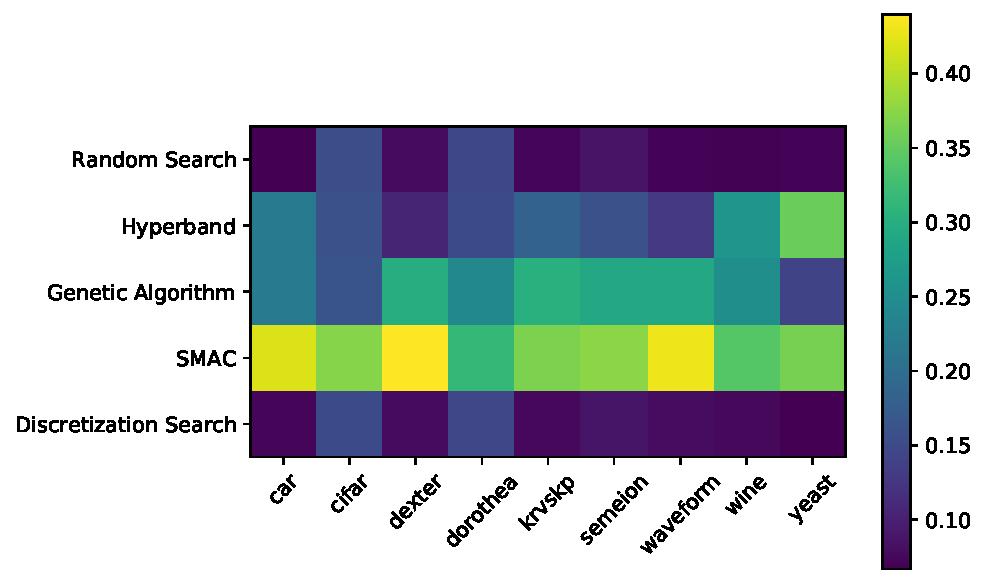
\includegraphics[width=\textwidth,keepaspectratio]{gfx/Figures/Evaluation/OptimizerCallsHeatmap.pdf}
    \end{subfigure}
\end{table}

After listing the relative optimizer utilization frequencies, this optimizer utilization is considered in the context of the different datasets and their properties in Tab.~\ref{table:optimizer-call-correlations}.
The following general dataset properties are gathered from OpenML for each dataset:
\begin{itemize}
    \item \textit{Instances}: The number of instances of the dataset.
    \item \textit{Features}: The number of features that each instance has.
    \item \textit{Classes}: The number of available target classes the instances are classified into.
    \item \textit{Dimensionality}: The relationship between features and instances that is calculated via \textit{Features} divided by \textit{Instances}.
    \item \textit{Autocorrelation}: After assigning consecutive numbers to the classes, the average difference of the classes for successive instances.
    \item \textit{Minority Class}: How much percent of \textit{Instances} is classified by the minority class.
    \item \textit{Majority Class}: How much percent of \textit{Instances} is classified by the majority class.
    \item \textit{Class Entropy}: Information theoretic entropy value of the class values.
\end{itemize}
These values are examined in terms of a correlation with the optimizer utilization of the five different optimization algorithms.
For the sake of completeness, this is here not only done for the relative frequency but also for the absolute frequency and rankings of the five optimizer utilization frequencies as well.\newline
Because linearity and an underlying normal distribution cannot be ensured, since the datasets were deliberately chosen to be very different from one another, the correlation coefficient has to be calculated with the non-parametric Spearman's rank correlation coefficient $\rho$.

\begin{table}[ht]
    \caption[Analysis of possible correlations between optimizer utilization and dataset properties.]{Analysis of possible correlations between optimizer utilization and dataset properties via the Spearman's rank correlation coefficient $\rho$ with four decimal places. RS = Random Search, HB = Hyperband, GA = Genetic Algorithm, DS = Discretization Search}
    \label{table:optimizer-call-correlations}
    \renewcommand{\arraystretch}{1.25}
    \begin{subtable}{\textwidth}
        \centering
        \caption{Relative utilization frequency.}
        \begin{tabular}{l|ccccc}
            & \textit{RS} & \textit{HB} & \textit{GA} & \textit{SMAC} & \textit{DS} \\
            \hline
            \textit{Instances} & $\phantom{-}0.0223$ & $\phantom{-}0.0051$ & $\phantom{-}0.0044$ & $\phantom{-}0.0080$ & $\phantom{-}0.0294$ \\
            \textit{Features} & $\phantom{-}0.2286$ & $-0.0560$ & $\phantom{-}0.1109$ & $\phantom{-}0.0087$ & $\phantom{-}0.2091$ \\
            \textit{Classes} & $-0.0275$ & $\phantom{-}0.0899$ & $-0.0780$ & $-0.0165$ & $-0.0208$ \\
            \textit{Dimensionality} & $\phantom{-}0.2027$ & $-0.0323$ & $\phantom{-}0.0903$ & $\phantom{-}0.0053$ & $\phantom{-}0.1799$ \\
            \textit{Autocorrelation} & $-0.0906$ & $-0.0621$ & $\phantom{-}0.0002$ & $-0.0508$ & $-0.0746$ \\
            \textit{Minority Class} & $\phantom{-}0.0643$ & $-0.1615$ & $\phantom{-}0.1050$ & $\phantom{-}0.0496$ & $\phantom{-}0.0494$ \\
            \textit{Majority Class} & $\phantom{-}0.0039$ & $-0.0224$ & $\phantom{-}0.0359$ & $-0.0081$ & $\phantom{-}0.0060$ \\
            \textit{Class Entropy} & $-0.0315$ & $\phantom{-}0.0476$ & $-0.0587$ & $-0.0053$ & $-0.0250$ \\
            \hline
        \end{tabular}
    \end{subtable}
    \par\bigskip
    \begin{subtable}{\textwidth}
        \centering
        \caption{Absolute utilization frequency.}
        \begin{tabular}{l|ccccc}
            & \textit{RS} & \textit{HB} & \textit{GA} & \textit{SMAC} & \textit{DS} \\
            \hline
            \textit{Instances} & $\phantom{-}0.0188$ & $\phantom{-}0.0155$ & $\phantom{-}0.0038$ & $\phantom{-}0.0179$ & $\phantom{-}0.0284$ \\
            \textit{Features} & $\phantom{-}0.0724$ & $-0.1501$ & $-0.0533$ & $-0.0782$ & $\phantom{-}0.0563$ \\
            \textit{Classes} & $\phantom{-}0.0349$ & $\phantom{-}0.1146$ & $\phantom{-}0.0026$ & $\phantom{-}0.0328$ & $\phantom{-}0.0482$ \\
            \textit{Dimensionality} & $\phantom{-}0.0660$ &$ -0.1232$ & $-0.0531$ & $-0.0714$ & $\phantom{-}0.0464$ \\
            \textit{Autocorrelation} & $\phantom{-}0.0084$ & $-0.0103$ & $\phantom{-}0.0254$ & $-0.0214$ & $\phantom{-}0.0075$ \\
            \textit{Minority Class} & $\phantom{-}0.0184$ & $-0.1662$ & $\phantom{-}0.0001$ & $-0.0006$ & $\phantom{-}0.0075$ \\
            \textit{Majority Class} & $-0.0730$ & $-0.0694$ & $-0.0276$ & $-0.0574$ & $-0.0762$ \\
            \textit{Class Entropy} & $\phantom{-}0.0496$ & $\phantom{-}0.0938$ & $\phantom{-}0.0214$ & $\phantom{-}0.0499$ & $\phantom{-}0.0619$ \\
            \hline
        \end{tabular}
    \end{subtable}
    \par\bigskip
    \begin{subtable}{\textwidth}
        \centering
        \caption{Optimizer utilization ranking.}
        \begin{tabular}{l|ccccc}
            & \textit{RS} & \textit{HB} & \textit{GA} & \textit{SMAC} & \textit{DS} \\
            \hline
            \textit{Instances} & $-0.0259$ & $\phantom{-}0.0030$ & $\phantom{-}0.0171$ & $\phantom{-}0.0202$ & $-0.0319$ \\
            \textit{Features} & $-0.0163$ & $\phantom{-}0.1286$ & $\phantom{-}0.0418$ & $\phantom{-}0.0279$ & $-0.0750$ \\
            \textit{Classes} & $-0.0043$ & $-0.0894$ & $\phantom{-}0.0673$ & $\phantom{-}0.0168$ & $-0.0065$ \\
            \textit{Dimensionality} & $-0.1409$ & $\phantom{-}0.0989$ & $\phantom{-}0.0432$ & $\phantom{-}0.0190$ & $-0.0520$ \\
            \textit{Autocorrelation} & $\phantom{-}0.0167$ & $\phantom{-}0.0548$ & $-0.0415$ & $-0.0074$ & $-0.0219$ \\
            \textit{Minority Class} & $-0.0745$ & $\phantom{-}0.1617$ & $-0.0381$ & $-0.0449$ & $-0.0273$ \\
            \textit{Majority Class} & $\phantom{-}0.0485$ & $\phantom{-}0.0253$ & $-0.0613$ & $\phantom{-}0.0047$ & $\phantom{-}0.0113$ \\
            \textit{Class Entropy} & $\phantom{-}0.0191$ & $-0.0541$ & $\phantom{-}0.0598$ & $\phantom{-}0.0043$ & $-0.0153$ \\
            \hline
        \end{tabular}
    \end{subtable}
\end{table}

The second evaluated aspect of frankensteins-automl's mechanics is the influence study of the two main components, i.e. model selection via MCTS and model configuration via the warmstarted optimizer ensembles.\newline
This is evaluated with the three variants of frankensteins-automl for three different timeouts in the context of 30 random seeds and the same nine datasets.
An analysis for significant improvement or deterioration within one timeout value is here done in the form of a Welch's \textit{t}-test with $p = 0.05$ as well.\newline
All accuracy score averages as well as the significance analysis results can be seen in Tab.~\ref{table:influence-results}.

\begin{table}[ht]
    \caption[Results of the experiments for comparing the three frankensteins-automl variants over longer timeouts.]{
        Results of the experiments for comparing the three frankensteins-automl variants over longer timeouts.
        The individual cells have the same layout as in Tab.~\ref{table:benchmark-results}.
    }
    \label{table:influence-results}
    \renewcommand{\arraystretch}{1.25}
    \begin{subtable}{\textwidth}
        \centering
        \caption{Timeout: 1h}
        \begin{tabular}{l|ccc}
            & \texttt{frankensteins-automl}  & \texttt{frankenstein-rs}  & \texttt{frankenstein-mcts} \\
            \hline
            \texttt{car} & $ 0.9789 \pm 0.0426 (30) \phantom{\downarrow}$ & $ \boldsymbol{0.9871} \pm 0.0148 (30) \phantom{\downarrow}$ & $ 0.9633 \pm 0.0674 (30) \phantom{\downarrow}$\\
            \texttt{cifar} & $ \boldsymbol{0.3140} \pm 0.0621 (28) \phantom{\downarrow}$ & $ 0.2841 \pm 0.0632 (28) \phantom{\downarrow}$ & $ 0.2664 \pm 0.0768 (30) \downarrow$\\
            \texttt{dexter} & $ 0.9004 \pm 0.0453 (28) \phantom{\downarrow}$ & $ 0.9020 \pm 0.0552 (28) \phantom{\downarrow}$ & $ \boldsymbol{0.9090} \pm 0.0426 (29) \phantom{\downarrow}$\\
            \texttt{dorothea} & $ \boldsymbol{0.9245} \pm 0.0136 (30) \phantom{\downarrow}$ & $ 0.9183 \pm 0.0235 (29) \phantom{\downarrow}$ & $ 0.9197 \pm 0.0140 (29) \phantom{\downarrow}$\\
            \texttt{krvskp} & $ \boldsymbol{0.9933} \pm 0.0023 (27) \phantom{\downarrow}$ & $ 0.9872 \pm 0.0301 (30) \phantom{\downarrow}$ & $ 0.9931 \pm 0.0025 (29) \phantom{\downarrow}$\\
            \texttt{semeion} & $ 0.9235 \pm 0.0588 (30) \phantom{\downarrow}$ & $ \boldsymbol{0.9317} \pm 0.0452 (30) \phantom{\downarrow}$ & $ 0.9221 \pm 0.0533 (30) \phantom{\downarrow}$\\
            \texttt{waveform} & $ 0.8412 \pm 0.0278 (29) \phantom{\downarrow}$ & $ \boldsymbol{0.8420} \pm 0.0313 (30) \phantom{\downarrow}$ & $ 0.8124 \pm 0.1066 (30) \phantom{\downarrow}$\\
            \texttt{wine} & $ 0.5292 \pm 0.1629 (28) \phantom{\downarrow}$ & $ 0.5709 \pm 0.1327 (27) \phantom{\downarrow}$ & $ \boldsymbol{0.6218} \pm 0.0890 (29) \uparrow$\\
            \texttt{yeast} & $ \boldsymbol{0.5752} \pm 0.0592 (30) \phantom{\downarrow}$ & $ 0.5594 \pm 0.0822 (28) \phantom{\downarrow}$ & $ 0.5323 \pm 0.0933 (29) \downarrow$\\
            \hline
        \end{tabular}
    \end{subtable}
    \par\bigskip
    \begin{subtable}{\textwidth}
        \centering
        \caption{Timeout: 6h}
        \begin{tabular}{l|ccc}
            & \texttt{frankensteins-automl}  & \texttt{frankenstein-rs}  & \texttt{frankenstein-mcts} \\
            \hline
            \texttt{car} & $ 0.9714 \pm 0.0577 (30) \phantom{\downarrow}$ & $ \boldsymbol{0.9926} \pm 0.0068 (30) \phantom{\downarrow}$ & $ 0.9729 \pm 0.0602 (30) \phantom{\downarrow}$\\
            \texttt{cifar} & $ 0.3048 \pm 0.0652 (30) \phantom{\downarrow}$ & $ 0.3025 \pm 0.0682 (29) \phantom{\downarrow}$ & $ \boldsymbol{0.3210} \pm 0.0542 (30) \phantom{\downarrow}$\\
            \texttt{dexter} & $ 0.8904 \pm 0.1030 (29) \phantom{\downarrow}$ & $ 0.9044 \pm 0.0600 (29) \phantom{\downarrow}$ & $ \boldsymbol{0.9222} \pm 0.0255 (29) \phantom{\downarrow}$\\
            \texttt{dorothea} & $ 0.9094 \pm 0.1078 (29) \phantom{\downarrow}$ & $ 0.9086 \pm 0.1108 (30) \phantom{\downarrow}$ & $ \boldsymbol{0.9218} \pm 0.0173 (30) \phantom{\downarrow}$\\
            \texttt{krvskp} & $ \boldsymbol{0.9930} \pm 0.0022 (29) \phantom{\downarrow}$ & $ 0.9920 \pm 0.0086 (30) \phantom{\downarrow}$ & $ 0.9926 \pm 0.0022 (30) \phantom{\downarrow}$\\
            \texttt{semeion} & $ 0.9070 \pm 0.1576 (30) \phantom{\downarrow}$ & $ \boldsymbol{0.9487} \pm 0.0206 (30) \phantom{\downarrow}$ & $ 0.9093 \pm 0.0860 (30) \phantom{\downarrow}$\\
            \texttt{waveform} & $ \boldsymbol{0.8500} \pm 0.0241 (30) \phantom{\downarrow}$ & $ 0.8480 \pm 0.0322 (29) \phantom{\downarrow}$ & $ 0.8362 \pm 0.0423 (30) \phantom{\downarrow}$\\
            \texttt{wine} & $ 0.6293 \pm 0.0985 (29) \phantom{\downarrow}$ & $ \boldsymbol{0.6510} \pm 0.0403 (28) \phantom{\downarrow}$ & $ 0.6326 \pm 0.0612 (30) \phantom{\downarrow}$\\
            \texttt{yeast} & $ 0.5759 \pm 0.0758 (30) \phantom{\downarrow}$ & $ 0.5697 \pm 0.0892 (30) \phantom{\downarrow}$ & $ \boldsymbol{0.5850} \pm 0.0648 (29) \phantom{\downarrow}$\\
            \hline
        \end{tabular}
    \end{subtable}
    \par\bigskip
    \begin{subtable}{\textwidth}
        \centering
        \caption{Timeout: 12h}
        \begin{tabular}{l|ccc}
            & \texttt{frankensteins-automl}  & \texttt{frankenstein-rs}  & \texttt{frankenstein-mcts} \\
            \hline
            \texttt{car} & $ 0.9838 \pm 0.0187 (30) \phantom{\downarrow}$ & $ \boldsymbol{0.9940} \pm 0.0057 (30) \uparrow$ & $ 0.9766 \pm 0.0556 (30) \phantom{\downarrow}$\\
            \texttt{cifar} & $ 0.3316 \pm 0.0467 (30) \phantom{\downarrow}$ & $ \boldsymbol{0.3319} \pm 0.0497 (30) \phantom{\downarrow}$ & $ 0.3069 \pm 0.0645 (30) \phantom{\downarrow}$\\
            \texttt{dexter} & $ 0.9265 \pm 0.0154 (30) \phantom{\downarrow}$ & $ \boldsymbol{0.9296} \pm 0.0128 (30) \phantom{\downarrow}$ & $ 0.9285 \pm 0.0127 (29) \phantom{\downarrow}$\\
            \texttt{dorothea} & $ \boldsymbol{0.9303} \pm 0.0136 (30) \phantom{\downarrow}$ & $ 0.9003 \pm 0.1494 (30) \phantom{\downarrow}$ & $ 0.9242 \pm 0.0205 (30) \phantom{\downarrow}$\\
            \texttt{krvskp} & $ 0.9928 \pm 0.0042 (30) \phantom{\downarrow}$ & $ \boldsymbol{0.9933} \pm 0.0025 (29) \phantom{\downarrow}$ & $ 0.9904 \pm 0.0113 (30) \phantom{\downarrow}$\\
            \texttt{semeion} & $ \boldsymbol{0.9501} \pm 0.0173 (30) \phantom{\downarrow}$ & $ 0.9411 \pm 0.0346 (30) \phantom{\downarrow}$ & $ 0.9498 \pm 0.0236 (30) \phantom{\downarrow}$\\
            \texttt{waveform} & $ 0.8547 \pm 0.0106 (30) \phantom{\downarrow}$ & $ \boldsymbol{0.8575} \pm 0.0165 (30) \phantom{\downarrow}$ & $ 0.8551 \pm 0.0095 (30) \phantom{\downarrow}$\\
            \texttt{wine} & $ \boldsymbol{0.6574} \pm 0.0404 (30) \phantom{\downarrow}$ & $ 0.6508 \pm 0.0793 (30) \phantom{\downarrow}$ & $ 0.6491 \pm 0.0764 (30) \phantom{\downarrow}$\\
            \texttt{yeast} & $ \boldsymbol{0.6028} \pm 0.0213 (30) \phantom{\downarrow}$ & $ 0.5995 \pm 0.0209 (29) \phantom{\downarrow}$ & $ 0.5981 \pm 0.0245 (30) \phantom{\downarrow}$\\
            \hline
        \end{tabular}
    \end{subtable}
\end{table}

\section{Analysis of the Experiment Outcomes}
\label{sec:evaluation:analysis}
This collected data is now analysed in more detail and used to answer the two main research questions of this thesis.

\subsection{Feasibility of AutoML via an Optimizer Ensembles}
\label{sec:evaluation:analysis:feasibility}
The first research question is about the feasibility of this optimizer ensembles approach for AutoML problems.\newline
As observed in Tab.~\ref{table:benchmark-results} and Tab.~\ref{table:significanse-counts}, this approach is partially competitive to the compared state-of-the-art approaches.
It appears for the evaluated datasets in large parts inferior to auto-sklearn mosaic, where it was only able to achieve competitive scores without a significant deterioration for two respectively three datasets but yields no significant improvements for any dataset.
Compared to ML-Plan and TPOT, the benchmark appears more balanced.
It shows a minor advantage compared to ML-Plan with significant improvements for five datasets and minor disadvantages compared to TPOT with significant improvements for only one dataset.\newline
Based on these results, the current reference implementation of the approach of this thesis shows no significant improvements against the established state-of-the-art approaches.
However, it was able to yield partially competitive results and this could indicate the ability to close up to the current state-of-the-art with further developments and refinements.

As part of the feasibility question, it is also evaluated which influences the two core components of this approach, i.e. model selection and optimizer selection as a Multi-Armed Bandit problem tackled via MCTS as well as model configuration approached with warmstarted optimizer ensembles, have on the results.
The results of this evaluation can be found in Tab.~\ref{table:influence-results}.\newline
For this experiment, one of the components is replaced with an alternative default behavior.
At first, a random search instead of MCTS but all optimizers included.
Second, only Bayesian optimization but reached via an MCTS.
Both were seen as competitors to the unmodified approach with an MCTS and all optimizers.\newline
Unfortunately, across all three evaluated timeouts, there are only four occurrences of one of the modified variants having significantly different scores compared to the unmodified and complete variant.
Additionally, these four significant differences do not suggest any kind of pattern and are most likely just outliers.\newline
Solely based on the evaluated datasets and timeouts, this data can be interpreted in two ways.
Either, the approach appears to be powered by a combination of both components and is not clearly influenced by one more than the other.
Alternatively, it is also possible that one of the more sophisticated components of this approach is not required and could be replaced by one of the simplified alternatives, random search instead of MCTS or only Bayesian optimization instead of optimizer ensembles.
A broader influence study is necessary to decide with interpretation is more accurate.

All in all, the current reference implementation does not indicate feasibility of the optimizer ensemble approach of this thesis under the constraints of the experiments.
It has to be noted, that these constraints prevented the approach from its ability to construct pipeline topologies with arbitrary size and complexity.
Additionally, the other approaches, especially auto-sklearn and TPOT, haven been in development for a significantly longer time and have therefore reached a much higher level of implementation maturity and code optimization.\newline
But since the results were at least partially competitive, it is not completely ruled out, that this idea can become feasible when this reference implementation has reached a comparable degree of maturity and optimization as auto-sklearn and TPOT and the some of the future work ideas are incorporated.\newline
The apparently similar influence of both components on the overall behavior does not give a clear suggestion, on which of these two components this future research should be focussed.
More evaluations and experimentation with modifications and additions in both components will be necessary.
Furthermore, this approach should be evaluated in an experimental setting where the pipeline topology and length are not constrained especially against other approaches that are able to construct such pipelines as well, i.e. ML-Plan and TPOT.

\subsection{Optimizer Utilization Frequencies}
\label{sec:evaluation:analysis:optimizer}
Since an MCTS as a method to tackle a Multi-Armed Bandit problem is used to select the optimizer, it will try to explore the most suitable optimizer for each problem class/instance and exploit it.
Hence, if the timeout is long enough and MCTS was able to perform a sufficient exploration, there should be a visible trend towards one or more optimizers for the problem class, i.e. an input dataset.\newline
This inherent mechanism of gathering indications about the suitability of an optimization algorithm towards the optimization of parametrizations of constructed pipelines for different datasets is the basis for the second research question.\newline
It should be examined if there are recognizable trends or tendencies towards one or more optimization algorithms across all datasets or otherwise if it is correlated to properties of the corresponding dataset which optimizer was utilized with which frequency.

As presented in Tab.~\ref{table:optimizer-calls}, SMAC, i.e. an implementation of Bayesian optimization, was utilized most often for each of the datasets.
Although Hyperband and the Genetic Algorithm came more or less close regarding the relative utilization frequency, they appear to be selected less favorably by the MCTS.
Both random search, as well as discretization search, trail significantly far behind the other three and have really low utilization frequency with a maximum of around $15\%$.\newline
If a ranking is created along with the five overall relative utilizations it would look like the following:
\begin{enumerate}
    \item SMAC
    \item Genetic Algorithm
    \item Hyperband
    \item Discretization Search
    \item Random Search
\end{enumerate}
This ranking is interesting in two ways.
First, since Hyperband is more or less a more sophisticated random search, the three least suitable optimization algorithms are all based on search algorithms.\newline
Second, auto-sklearn as well as Mosaic use internally Bayesian Optimization, TPOT a genetic algorithm, and ML-Plan a more complex form of Discretization Search.
When this ranking is now compared to the results of these four AutoML approaches in Tab.~\ref{table:benchmark-results}, there is a similarity to be observed as auto-sklearn, Mosaic, and TPOT being at the top with comparable scores, but clearly superior to ML-Plan for the evaluated datasets in this experiment series.
Theoretically, this would be another match of findings for the benchmark scores in comparison to the optimizer utilization ranking.
But this is probably all in all solely a coincidence and not caused by the actual choice of optimization algorithm, because the three approaches perform more competitive in other benchmark evaluations with longer timeouts~\cite{Mohr-ML-Plan} than in this evaluation.

Since there is a clear trend recognizable regarding the most favorable optimizer choices of the MCTS across all datasets of this experiment, the evaluation regarding correlations between dataset properties and optimizer utilization becomes less relevant but is done nevertheless.\newline
As presented in Tab.~\ref{table:influence-results}, there are only weak correlation coefficients between all dataset properties and optimizer utilization across all three utilization metrics.
The correlation coefficients are overall in the range $-0.1662 \leq \rho \leq 0.2286$, which does not suggest any significant correlation altogether.

These interpreted results suggest that SMAC is the most suitable choice of optimization algorithm across all regarded datasets independently of the eight evaluated dataset properties.
If this is a trend beyond the scope of this evaluation, has to be controlled in an evaluation with a much higher amount of different datasets.
